\chapter{相关工作}
\section{程序间差异分析}

对于软件演进分析而言,如何确定一个程序的不同版本之间的变更是一个关键性的问题\cite{kim2013identifying}。程序间差异分析能够通过分析同一程序的不同版本间的差异,来确定版本间的变更集合\cite{lahiri2010differential,winstead2003towards}。

按分析的深度而言,程序间差异分析可以分为三类:
\begin{itemize}
	\item 文本差异:单纯对比文本间的不同,这是最简单也最广泛应用的分析方法,如Unix Diff工具。
	\item 语法差异:对比并获得源代码间语法结构上的不同。
	\item 语义差异:对比并获得源代码间语义层面上的不同。
\end{itemize}

现有的帮助工程师进行软件维护和演进活动的工具往往都受限于低质量的变更信息。例如源代码的变更信息往往都存储于版本管理系统中,如CVS等。他们会追踪对某个特定文件的文本行的增加/删除等操作,并没有考虑代码中的结构化变更。

考虑到源代码可以抽象语法树(Abstract Syntax Tree)的形式进行表达,可以考虑采用树间差异分析的方法来抽取出这些变更信息。Change Distilling就是这样一类进行树间差异分析的算法\cite{fluri2007change,gall2009change}。该算法能够从两棵AST之间寻找匹配节点,并找到一个能够令一棵树转化为另一棵树的最小变更集合,该变更集合即为所求的程序间差异。而且由于是从AST的实体和语句中抽取信息,该算法可以获取结构化的变更信息。

Change Distilling中采用二元字符串相似性来匹配源代码语句,并使用子树相似性来匹配源代码结构(如语句、循环等)。在寻找变更集合时,它采用基本的树变更操作来描述源代码的变更,包括更新、删除、增加等。在实际的使用过程中,该算法可能会受限于如何找到合适数量的移动操作。

\section{程序变更影响分析}
软件维护是软件开发周期中最复杂、高成本和劳动密集的活动。软件产品天然的需要跟随系统需求的变更而进行适应和变化,以满足用户的需求。软件变更是软件维护中的基础组件。变更可能从新的需求、缺陷修复、变更请求等而来,当变更应用于软件时,他们不可避免的会带来一些副作用,也可能会与原软件的其他部分产生不协调。

而CIA正是这样一类用于确定变更对于软件其他部分的影响的技术集合\cite{li2013survey},它在软件开发、维护和回归测试等过程中都起到着重要的作用\cite{acharya2011practical}。一般而言,CIA可以用于程序理解、变更影响预测、影响追踪、变更传播、测试用例的选取等。

CIA方法的分类:
\begin{itemize}
	\item 基于追踪性的CIA\cite{de2008traceability},追踪两个不同抽象级别上的元素间的依赖性,目的在于链接不同类型的软件工件(需求、设计等)。

	\item 基于依赖关系的CIA\cite{law2003incremental},致力于衡量变更的潜在影响,通常尝试去分析程序的语法关系,他们表示了程序实体间的一些语义依赖关系,或者说他们在同一个抽象级别上对软件工件实施了影响分析。现在最主要的这类CIA主要在源代码级别上进行研究。
\end{itemize}

软件系统上的变更可能导致不可意料的副作用,CIA的目标就在于辨认这些副作用(side effect或者ripple effect)\cite{bohner1996software},并防止之。
CIA从分析变更请求和源代码开始,以便获得变更集合(change set)。最后实际获得的影响集合叫做EIS(estimated impact set),而真实的集合叫做AIS(actual impact set)。

整个软件变更影响的分析过程可以大致分为以下流程,更详细的流程可以参考图2.3\cite{de2008traceability,bohner2002software}。

\begin{enumerate}
	\item 确定变更集合,需要针对变更请求进行分析,这步一般叫做特征定位(feature location),用于确认源代码中实现了对应功能的起始位置\cite{biggerstaff1993concept}。
	\item 衡量由变更集合引入的影响。这一步是目前大部分CIA技术的着重点。若按分析技术的类型划分,则主要的两类包括静态分析和动态分析。
	\begin{itemize}
	
	\item 静态分析:历史分析、文本分析、结构分析\cite{sun2012comparative,kagdi2007survey}。静态分析通过分析程序的语法、语义或者历史依赖实现,通常会产生很多错报(False Positive)。
		\begin{itemize}
		\item 结构分析着重于分析程序的结构依赖性,构建依赖关系图
		\item 文本分析根据注释和标识符提取出概念依赖性
		\item 历史分析从多个软件演进版本中挖掘出信息
		\end{itemize}
		\begin{figure}[H]
			\centering
			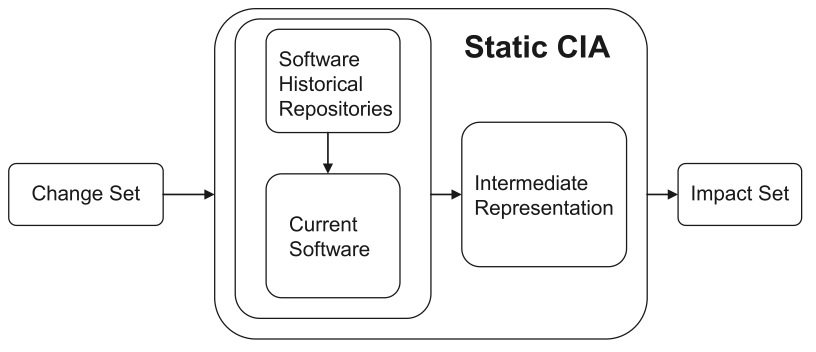
\includegraphics{chap02_02}
			\caption {静态分析过程}
		\end{figure}
	
	\item 动态分析:在线分析和离线分析。考虑特定的输入,并且依赖于程序运行时收集到的信息进行分析(如运行时的追踪信息、覆盖信息等)\cite{law2003whole}。其得到的影响集合往往比静态分析精度更高,但其开销也相应更大,而且通常包括错报(False Negative)。
		\begin{itemize}
		\item 在线CIA使用程序运行时收集的信息实施所有的分析
		\end{itemize}
		
		\begin{figure}[H]
			\centering
			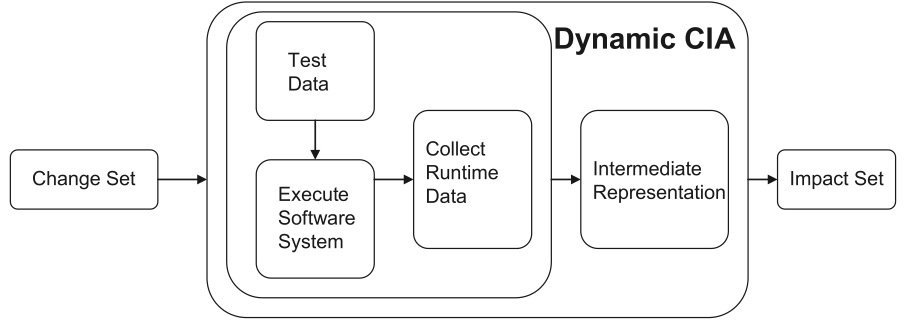
\includegraphics{chap02_03}
			\caption {动态分析过程}
		\end{figure}	

		
	\end{itemize}
\end{enumerate}


近年来,涌现出一些以CIA技术作为支撑而实现的工具,它们一般在实现CIA技术之后,利用得到的影响集合进行后续分析,帮助进行软件维护和演进。下面对它们进行简要的介绍:
\begin{enumerate}
	\item Chianti:应用于Java程序,Eclipse插件\cite{ren2004chianti}。

	它可以:
	\begin{enumerate}
	
		\item 使用回归测试来分析变更之前的程序功能是否能正常使用。
		\item 若测试失败,利用Chianti进行变更影响分析,将软件变更拆分成若干原子变更,并分析他们之间的依赖关系,结合原程序生成中间表示形式,分析可能是哪些部分影响到了测试用例的运行。
	\end{enumerate}
	
	
	\item JRipples:应用于Java程序,Eclipse插件\cite{buckner2005jripples,rajlich2004incremental}。
	
	它利用依赖关系图,自动标注可能受到被变更的类所影响的其他类,并向用户展示其变更的影响传播路径。可利用人工标注来修正结果。
	
	\item ROSE:应用于Java CVS工程,Eclipse插件\cite{zimmermann2005mining}。

	它可以挖掘软件代码仓库,当用户对代码变更时提示用户可能相关的变更(类似于“变更了这个函数的人通常还变更了另一个函数”)。
	
	
	\item jpf-regression:应用于Java程序,Eclipse插件或命令行工具\cite{person2011directed}。

	它可以利用程序切片技术进行变更影响分析,利用得到的影响集合来驱动符号化执行,获取被改变部分代码的行为。
\end{enumerate}

\begin{figure}[H]
	\centering
	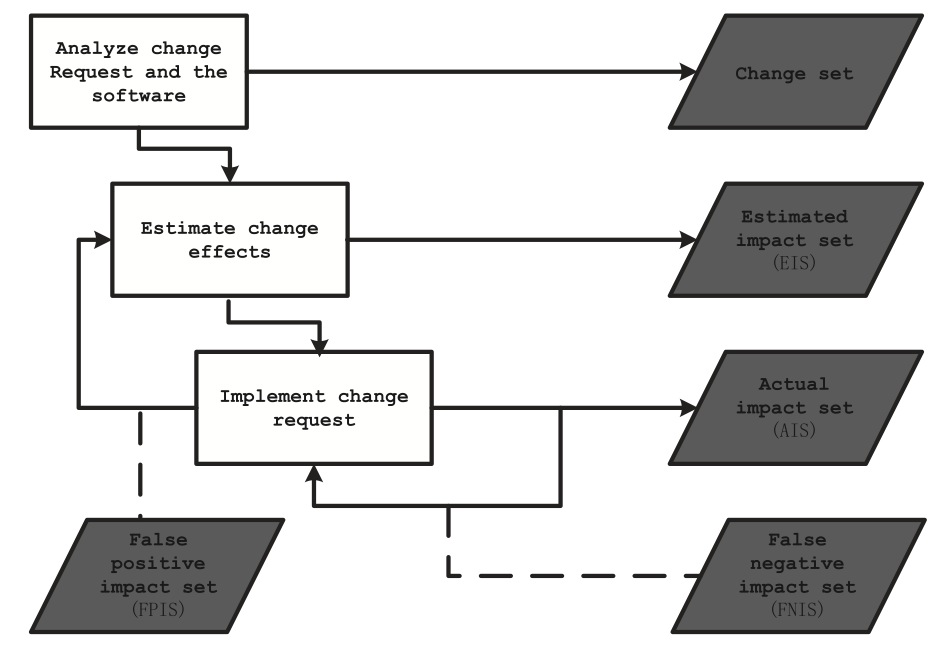
\includegraphics[width=.8\columnwidth]{chap02_01}
	\caption {CIA过程}
\end{figure}

\section{相关工具}
	本节将主要介绍本文中采用到的相关工具。
	

	\subsection{git}		

git是一个分布式的版本控制系统,最初由 Linus Torvalds在2005年为Linux内核而开发,现在已经成为最流行的版本控制系统。

与CVS和SVN等集中式的C/S版本控制系统不同,git是分布式的版本库,每个本地的git工作目录都包含了完整的历史数据和版本追踪能力,无需网络连接或服务器端。
      

本文中主要考虑以git作为版本管理系统的应用场景,类似于GitHub,假定为项目开发了new version和patch version两个不同的分支,并使用git的分支合并策略实现补丁的版本迁移过程。
	\subsection{Beyond Compare}
		
Beyond Compare 是一款内容比较工具,可以用于文件、目录、压缩包的比较,横跨Windows、Mac OS X、Linux三大操作系统,可用作版本控制系统的文本比较和合并工具,例如git。
      
本文中主要采用其作为git的文本比较和合并工具,用于解决补丁版本迁移时的冲突问题。


	\subsection{jpf-regression} 
变更影响分析常用于衡量软件变更的潜在影响。CIA的结果通常可用做其他程序分析技术的输入,例如回归测试可利用CIA来确定程序的哪些部分需要进行再分析。而由于软件开发过程的演进特性,并且软件系统的大小和复杂性越来越高,刺激了人们对于有效的变更影响分析的需求。\cite{rungta2012change}

一般而言,“单行变更”就足以引发广泛而未知的影响,因而变更影响分析在软件演进和维护过程中扮演着重要的作用。

目前,大部分的自动分析工具都将变更的影响以程序句法结构的形式表现出来,例如函数和程序语句。基于依赖的分析方法则通过分析程序组件间的内部关系来衡量变更的影响。这类技术能够以程序位置信息来描述变更的影响,然而却缺失了与受影响位置相关的程序运行路径的信息,而这类信息往往对于程序行为的验证、调试等起到很大的作用,而且能够将关注的范围缩小,只关注受到影响的程序行为集合。

(Directed Incremental Symbolic Execution )DiSE\cite{person2011directed,yang2014directed}能够结合静态分析的效率和符号化执行的精度,分析方法内部的变更影响,并描述程序变更对其运行行为的影响。

DiSE的静态分析部分采用程序切片技术来衡量变更对代码中其他位置的影响,其生成的影响集合可以用于引导符号化执行去分析受到影响的程序行为,并生成对应的路径条件(path condition),这些路径条件用于描述受到影响的程序行为。这些路径条件之后可以利用SMT等技术进行求解,用于后续的验证、调试等过程。

在DiSE方法中,程序变更影响分析是其进行后续分析过程的基础,它的变更影响分析过程主要特点在于:
\begin{enumerate}
	\item 粒度:语句级别。即具体的影响分析过程中,以程序语句为基本单位进行影响集合的计算。
	\item 影响范围:方法内部。即以方法的作用域作为单次影响集合计算的限制范围,最后得到变更对其所处的方法内部其他语句所造成的影响。也就是说不计算变更对于其他方法的影响,即不考虑对方法内部函数调用的影响。
	\item 影响来源:主要从控制流和数据流两个层面考虑变更所造成的影响,实际上采用了语句间的控制依赖和数据依赖关系进行计算。
\end{enumerate}

DiSE中,受影响的集合主要分为两类:
\begin{itemize}
	\item ACN:受影响的条件语句节点(affected conditional nodes)。
	\item AWN:受影响的赋值语句节点(affected write nodes)。
\end{itemize}

为了计算得到这两类影响集合,DiSE中一共使用了四条规则来迭代计算,从最初的变更集合出发,不断应用规则向外扩展,最后计算得到闭包,即为所求的影响集合:
\begin{enumerate}
	\item 如果ACN中有一个节点$n_i$,且存在一个条件节点$n_j$,其中$n_j$控制依赖于$n_i$,那么将$n_j$加入到ACN中。
	\item 如果nj是一条赋值语句,且控制依赖于ACN中的节点$n_i$,那么$n_j$加入到AWN中。
	     
	前两条公式表明,如果条件语句和赋值语句控制依赖于变更后的CFG中的节点,那么他们就应当被加进来。
	     
	\item 如果AWN中的一条赋值语句节点$n_i$对于变量的赋值在条件语句$n_j$中被使用了,且CFG中存在一条从$n_i$到$n_j$的路径,那么将$n_j$加入到ACN中。

	\item 如果一个写语句节点$n_i$对于对于变量的赋值在AWN或ACN中的某个节点$n_j$被使用了,且CFG中存在一条从$n_i$到$n_j$的路径,那么将$n_i$加入到AWN中。

\end{enumerate}

jpf-regression是DiSE的工具实现,它是基于Java Path Finder框架\cite{havelund2000mode}而实现的工具,可作为Eclipse的插件使用,支持Java语言。

\subsection{ASTro}	

	本文中所采用的AST比较工具是由内布拉斯加大学林肯分校的Josh Reed,Suzette Person和Sebastian Elbaum等人所开发的ASTro,它也是jpf-regression中使用的前置工具,用于对比两个不同版本的源代码,并获取其抽象语法树上的差异,以XML文件的格式进行输出。该工具支持Java语言。
	